%
% chapter.tex -- Kapitel mit den Grunddefinition und Notationen
%
% (c) 2020 Prof Dr Andreas Müller, OST Ostschweizer Fachhochschule
%
\chapter{Zahlen
\label{buch:chapter:zahlen}}
\lhead{Zahlen}
\rhead{}

Das Thema dieses Buches ist die Konstruktion interessanter 
mathematischer Objekte mit Hilfe von Matrizen.
Die Einträge dieser Matrizen sind natürlich Zahlen.
Wir wollen von den bekannten Zahlmengen als grundlegenden
Bausteinen ausgehen.
Dies schliesst natürlich nicht aus, dass man auch Zahlenmengen
mit Hilfe von Matrizen beschreiben kann, wie wir es später für die
komplexen Zahlen machen werden.

In diesem Kapitel sollen daher die Eigenschaften der bekannten
Zahlensysteme der natürlichen, ganzen, rationalen, reellen und
komplexen Zahlen nochmals in einer Übersicht zusammengetragen
werden.
Dabei wird besonderes Gewicht darauf gelegt, wie in jedem Fall
einerseits neue Objekte postuliert, andererseits
aber auch konkrete Objekte konstruiert werden können.

%
% natuerlich.tex
%
% (c) 2021 Prof Dr Andreas Müller, OST Ostschweizer Fachhochschule
%
% !TeX spellcheck = de_CH
\section{Natürliche Zahlen
\label{buch:section:natuerliche-zahlen}}
\rhead{Natürliche Zahlen}
Die natürlichen Zahlen sind die Zahlen, mit denen wir zählen.
\index{natürliche Zahlen}%
\index{N@$\mathbb{N}$}%
Sie abstrahieren das Konzept der Anzahl der Elemente einer endlichen
Menge.
Da die leere Menge keine Elemente hat, muss die Menge der natürlichen
Zahlen auch die Zahl $0$ enthalten.
Wir schreiben
\[
\mathbb{N}
=
\{
0,1,2,3,\dots
\}.
\]

\subsubsection{Peano-Axiome}
\index{Peano}%
Man kann den Zählprozess durch die folgenden Axiome von Peano genauer fassen:
\index{Peano-Axiome}%
\begin{enumerate}
\item $0$ ist eine natürliche Zahl: $0\in\mathbb N$.
\item Jede Zahl $n\in \mathbb{N}$ hat einen {\em Nachfolger}
$n'\in \mathbb{N}$.
\index{Nachfolger}%
\item $0$ ist nicht Nachfolger einer Zahl.
\item Wenn zwei Zahlen $n,m\in\mathbb{N}$ den gleichen Nachfolger haben,
$n'=m'$, dann sind sie gleich: $n=m$.
\item Enthält eine Menge $X$ die Zahl $0$ und mit jeder Zahl auch ihren
Nachfolger, dann ist $\mathbb{N}\subset X$.
\end{enumerate}

\subsubsection{Vollständige Induktion}
Es letzte Axiom formuliert das Prinzip der {\em vollständigen Induktion}.
\index{vollständige Induktion}%
\index{Induktion, vollständige}%
Um eine Aussage $P(n)$ für alle natürlichen Zahlen $n$
mit vollständiger Induktion zu beweisen, bezeichnet man mit
$X$ die Menge aller Zahlen, für die $P(n)$ wahr ist.
Die Induktionsverankerung beweist, dass $P(0)$ wahr ist, dass also $0\in X$.
Der Induktionsschritt beweist, dass mit einer Zahl $n\in X$ auch der
Nachfolger $n'\in X$ ist.
Nach dem letzten Axiom ist $\mathbb{N}\subset X$, oder anders ausgedrückt,
die Aussage $P(n)$ ist wahr für jede natürliche Zahl.

\subsubsection{Addition}
Aus der Nachfolgereigenschaft lässt sich durch wiederholte Anwendung
die vertrautere Addition konstruieren.
\index{Addition!in $\mathbb{N}$}%
Um die Zahl $n\in\mathbb{N}$ um $m\in\mathbb{N}$ zu vermehren, also
$n+m$ auszurechnen, kann man die rekursiven Regeln
\begin{align*}
n+0&=n\\
n+m'&=(n+m)'
\end{align*}
festlegen.
Nach diesen Regeln ist
\[
5+3
=
5+2'
=
(5+2)'
=
(5+1')'
=
((5+1)')'
=
((5+0')')'
=
(((5)')')'.
\]
Dies ist genau die Art und Weise, wie kleine Kinder rechnen lernen.
Sie zählen von $5$ ausgehend um $3$ weiter, manchmal unter Zuhilfenahme
ihrer Finger.
Der dritte Nachfolger von $5$ heisst üblicherweise $8$.

Die algebraische Struktur, die hier konstruiert worden ist, heisst
ein {\em Monoid}.
\index{Monoid}%
Allerdings kann man darin zum Beispiel nur selten Gleichungen
lösen, so etwa hat $3+x=1$ keine Lösung.
Die Addition ist nicht immer umkehrbar.

\subsubsection{Multiplikation}
Es ist klar, dass auch die Multiplikation definiert werden kann, 
sobald die Addition definiert ist.
Die Rekursionsformeln
\begin{align}
n\cdot 0 &= 0 \notag \\
n\cdot m' &= n\cdot m + n
\label{buch:zahlen:multiplikation-rekursion}
\end{align}
legen jedes Produkt von natürlichen Zahlen fest, zum Beispiel
\[
5\cdot 3
=
5\cdot 2'
=
5\cdot 2 + 5
=
5\cdot 1' + 5
=
5\cdot 1 + 5 + 5
=
5\cdot 0' + 5 + 5
=
5\cdot 0 + 5 + 5 + 5
=
5 + 5 + 5.
\]
Doch auch bezüglich der Multiplikation ist $\mathbb{N}$ unvollständig,
die Beispielgleichung $3x=1$ hat keine Lösung in $\mathbb{N}$.

\subsubsection{Rechenregeln}
Aus den Definitionen lassen sich auch die Rechenregeln ableiten,
die man für die alltägliche Rechnung braucht.
Zum Beispiel kommt es nicht auf die Reihenfolge der Summanden
oder Faktoren an. 
Das {\em Kommutativgesetz} besagt
\[
a+b=b+a
\qquad\text{und}\qquad
a\cdot b = b\cdot a.
\]
\index{Kommutativgesetz}%
Die Kommutativität der Addition werden wir auch in allen weiteren
Konstruktionen voraussetzen.
Die Kommutativität des Produktes ist allerdings weniger selbstverständlich
und wird beim Matrizenprodukt nur noch für spezielle Faktoren zutreffen.

Eine Summe oder ein Produkt mit mehr als zwei Summanden bzw.~Faktoren
kann in jeder beliebigen Reihenfolge ausgewertet werden,
\[
(a+b)+c
=
a+(b+c)
\qquad\text{und}\qquad
(a\cdot b)\cdot c
=
a\cdot (b\cdot c),
\]
dies ist das {\em Assoziativgesetz}.
Es gestattet auch eine solche Summe oder ein solches Produkt einfach
als $a+b+c$ bzw.~$a\cdot b\cdot c$ zu schreiben, da es ja keine Rolle
spielt, in welcher Reihenfolge man die Teilprodukte berechnet.

Die Konstruktion der Multiplikation als iterierte Addition mit Hilfe
der Rekursionsformel \eqref{buch:zahlen:multiplikation-rekursion}
hat auch zur Folge, dass die {\em Distributivgesetze}
\index{Distributivgesetz}%
\[
a\cdot(b+c) = ab+ac
\qquad\text{und}\qquad
(a+b)\cdot c = ac+bc
\]
gelten.
Bei einem nicht kommutativen Produkt ist es notwendig,
zwischen Links- und Rechtsdistributivgesetz zu unterscheiden.

Die Distributivgesetze drücken die wohlbekannte Regel des
Ausmultiplizierens aus.
Ein Distributivgesetz ist also grundlegend dafür, dass man mit den
Objekten so rechnen kann, wie man das in der elementaren Algebra 
gelernt hat.
Auch die Distributivgesetze sind daher Rechenregeln, die wir in
Zukunft immer dann fordern werden, wenn Addition und Multiplikation
definiert sind.
Sie gelten immer für Matrizen.

\subsubsection{Teilbarkeit}
Die Lösbarkeit von Gleichungen der Form $ax=b$ mit $a,b\in\mathbb{N}$
gibt Anlass zum sehr nützlichen Konzept der Teilbarkeit.
\index{Teilbarkeit}%
Die Zahl $b$ heisst {\em teilbar} durch $a$, in Formeln $a|b$,
wenn die Gleichung $ax=b$ eine Lösung in $\mathbb{N}$ hat.
\index{teilbar}%
Jede natürlich Zahl $n$ ist durch $1$ und durch sich selbst teilbar,
denn $n\cdot 1 = n$.
Andere Teiler sind dagegen nicht selbstverständlich.
Die Zahlen
\[
\mathbb{P}
=
\{2,3,5,7,11,13,17,19,23,29,\dots\}
\]
haben keine weiteren Teiler. Sie heissen {\em Primzahlen}.
\index{Primzahl}%
Die Menge der natürlichen Zahlen wird mit der Teilbarkeit zur naheliegenden
Arena für die Zahlentheorie.
\index{Zahlentheorie}%

\subsubsection{Konstruktion der natürlichen Zahlen aus der Mengenlehre}
Die Peano-Axiome postulieren, dass es natürliche Zahlen gibt.
Es werden keine Anstrengungen unternommen, die natürlichen Zahlen
aus noch grundlegenderen mathematischen Objekten zu konstruieren.
Die Mengenlehre bietet eine solche Möglichkeit.

Da die natürlichen Zahlen das Konzept der Anzahl der Elemente einer
Menge abstrahieren, gehört die leere Menge zur Zahl $0$.
Die Zahl $0$ kann also durch die leere Menge $\emptyset = \{\}$
wiedergegeben werden.

Der Nachfolger muss jetzt als eine Menge mit einem Element konstruiert
werden.
Das einzige mit Sicherheit existierende Objekt, das für diese Menge
zur Verfügung steht, ist $\emptyset$.
Zur Zahl $1$ gehört daher die Menge $\{\emptyset\}$, eine Menge mit
genau einem Element.
Stellt die Menge $N$ die Zahl $n$ dar, dann können wir die zu $n+1$
gehörige Menge $N'$ dadurch konstruieren, dass wir zu den Elemente
von $N$ ein zusätzliches Element hinzufügen, das noch nicht in $N$ ist,
zum Beispiel $\{N\}$:
\[
N' = N \cup \{ N \}.
\]

Die natürlichen Zahlen existieren also, wenn wir akzeptieren, dass es
Mengen gibt.
Die natürlichen Zahlen sind dann nacheinander die Mengen
\begin{align*}
0 &= \emptyset 
\\
1 &= 0 \cup \{0\} = \emptyset \cup \{0\} = \{0\}
\\
2 &= 1 \cup \{1\} = \{0\}\cup\{1\} = \{0,1\}
\\
3 &= 2 \cup \{2\} = \{0,1\}\cup \{2\} = \{0,1,2\}
\\
&\phantom{n}\vdots
\\
n+1&= n \cup \{n\} = \{0,\dots,n-1\} \cup \{n\} = \{0,1,\dots,n\}
\\
&\phantom{n}\vdots
\end{align*}
Die Menge $n+1$ besteht also aus den $n+1$ Zahlen von $0$ bis $n$.

Für spätere Verwendung in Kapitel~\ref{buch:chapter:permutationen}
definieren wir hier auch noch eine weiter Art von Standardteilmengen
von $\mathbb{N}$.

\begin{definition}
\label{buch:zahlen:def:[n]}
Die Menge $[n]\subset \mathbb{N}$ ist definiert durch
\[
[n] = \begin{cases}
\{1,2,\dots,n\}&\qquad \text{für $n>0$}\\
\emptyset&\qquad\text{für $n=0$}
\end{cases}
\]
\end{definition}

Jede der Mengen $[n]$ hat genau $n$ Elemente: $|[n]|=n$.

\subsubsection{Natürliche Zahlen als Äquivalenzklassen}
Im vorangegangenen Abschnitt haben wir die natürlichen Zahlen aus
der leeren Menge schrittweise sozusagen ``von unten'' aufgebaut.
Wir können aber auch eine Sichtweise ``von oben'' einnehmen.
Dazu definieren wir, was eine endliche Menge ist und was es heisst,
dass endliche Mengen gleiche Mächtigkeit haben.

\begin{definition}
Eine Menge $A$ heisst {\em endlich}, wenn es jede injektive Abbildung
$A\to A$ auch surjektiv ist.
\index{endlich}%
Zwei endliche Mengen $A$ und $B$ heissen {\em gleich mächtig},
\index{gleich mächtig}%
in Zeichen $A\sim B$, wenn es eine Bijektion
$A\to B$ gibt.
\end{definition}

Der Vorteil dieser Definition ist, dass sie die früher definierten 
natürlichen Zahlen nicht braucht, diese werden jetzt erst konstruiert.
Dazu fassen wir in der Menge aller endlichen Mengen die gleich mächtigen
Mengen zusammen, bilden also die Äquivalenzklassen der Relation $\sim$.
\index{Aquivalenzklasse@Äquivalenzklasse}%

Der Vorteil dieser Sichtweise ist, dass die natürlichen Zahlen ganz
explizit als die Anzahlen von Elementen einer endlichen Menge entstehen.
Eine natürlich Zahl ist also eine Äquivalenzklasse
$\llbracket A\rrbracket$, die alle endlichen Mengen enthält,  die die
gleiche Mächtigkeit wie $A$ haben.
Zum Beispiel gehört dazu auch die Menge, die im vorangegangenen
Abschnitt aus der leeren Menge aufgebaut wurde.

Die Mächtigkeit einer endlichen Menge $A$ ist die Äquivalenzklasse, in der
die Menge drin ist: $|A| = \llbracket A\rrbracket\in \mathbb{N}$ nach 
Konstruktion von $\mathbb{N}$.
Aus logischer Sicht etwas problematisch ist allerdings, dass wir 
von der ``Menge aller endlichen Mengen'' sprechen ohne uns zu versichern,
dass dies tatsächlich eine zulässige Konstruktion ist.


%
% ganz.tex -- Ganze Zahlen
%
% (c) 2021 Prof Dr Andreas Müller, OST Ostschweizer Fachhochschule
%
% !TeX spellcheck = de_CH
\section{Ganze Zahlen
\label{buch:section:ganze-zahlen}}
\rhead{Ganze Zahlen}
Die Menge der ganzen Zahlen löst das Problem, dass nicht jede
Gleichung der Form $x+a=b$ mit $a, b \in \mathbb N$
eine Lösung $x \in \mathbb N$ hat.
Dazu ist erforderlich, den natürlichen Zahlen die negativen Zahlen
hinzuzufügen, also wieder die Existenz neuer Objekte zu postulieren,
die die Rechenregeln weiterhin erfüllen.

\subsubsection{Paare von natürlichen Zahlen}
Die ganzen Zahlen können konstruiert werden als Paare $(u,v)$ von 
natürlichen Zahlen $u,v\in\mathbb{N}$.
Die Paare der Form $(u,0)$ entsprechen den natürlichen Zahlen, die
Paare $(0,v)$ sind die negativen Zahlen.
Die Rechenoperationen sind wie folgt definiert:
\begin{equation}
\begin{aligned}
(a,b)+(u,v) &= (a+u,b+v)
\\
(a,b)\cdot (u,v) &= (au+bv,av+bu)
\end{aligned}
\label{buch:zahlen:ganze-rechenregeln}
\end{equation}

\subsubsection{Äquivalenzrelation}
Die Definition~\eqref{buch:zahlen:ganze-rechenregeln}
erzeugt neue Paare, die wir noch nicht interpretieren können.
Zum Beispiel ist $0=1+(-1) = (1,0) + (0,1) = (1,1)$.
Die Paare $(u,u)$ müssen daher alle mit $0$ identifiziert werden.
Es folgt dann auch, dass alle Paare von natürlichen Zahlen mit 
``gleicher Differenz'' den gleichen ganzzahligen Wert darstellen,
allerdings können wir das nicht so formulieren, da ja die Differenz
noch gar nicht definiert ist.
Stattdessen gelten zwei Paare als äquivalent, wenn
\begin{equation}
(a,b) \sim (c,d)
\qquad\Leftrightarrow\qquad
a+d = c+b
\label{buch:zahlen:ganz-aquivalenz}
\end{equation}
gilt.
Diese Bedingung erhält man, indem man zu $a-b=c-d$ die Summe $b+d$ 
hinzuaddiert.
Ein ganzen Zahl $z$ ist daher eine Menge von Paaren von natürlichen
Zahlen mit der Eigenschaft
\[
(a,b)\in z\;\wedge (a',b')\in z
\qquad\Leftrightarrow\qquad
(a,b)\sim(a',b')
\qquad\Leftrightarrow\qquad
a+b' = a'+b.
\]
Man nennt eine solche Menge eine {\em Äquivalenzklasse} der Relation $\sim$.

Die Menge $\mathbb{Z}$ der {\em ganzen Zahlen} ist die Menge aller solchen
Äquivalenzklassen.
Die Menge der natürlichen Zahlen $\mathbb{N}$ ist in evidenter Weise
darin eingebettet als die Menge der Äquivalenzklassen von Paaren der
Form $(n,0)$.

\subsubsection{Entgegengesetzter Wert}
Zu jeder ganzen Zahl $z$ dargestellt durch das Paar $(a,b)$ 
stellt das Paar $(b,a)$ eine ganze Zahl dar mit der Eigenschaft
\begin{equation}
z+(b,a)
=
(a,b) + (b+a) = (a+b,a+b) \sim (0,0) = 0.
\label{buch:zahlen:eqn:entgegengesetzt}
\end{equation}
Die von $(b,a)$ dargestellte ganze Zahl wird mit $-z$ bezeichnet,
die Rechnung~\eqref{buch:zahlen:eqn:entgegengesetzt} lässt sich damit
abgekürzt als $z+(-z)=0$ schreiben.

\subsubsection{Lösung von Gleichungen}
Gleichungen der Form $a=x+b$ können jetzt für beliebige ganze Zahlen
immer gelöst werden.
Dazu schreibt man $a,b\in\mathbb{N}$ als Paare und sucht die
Lösung in der Form $x=(u,v)$.
Man erhält
\begin{align*}
(a,0) &= (u,v) + (b,0)
\\
(a+b,b) &= (u+b,v)
\end{align*}
Das Paar $(u,v) = (a,b)$ ist eine Lösung, die man normalerweise als
$a-b = (a,0) + (-(b,0)) = (a,0) + (0,b) = (a,b)$ schreibt.

\subsubsection{Ring}
\index{Ring}%
Die ganzen Zahlen sind ein Beispiel für einen sogenannten Ring,
eine algebraische Struktur in der Addition, Subtraktion und
Multiplikation definiert sind.
Weitere Beispiel werden später vorgestellt,
der Ring der Polynome $\mathbb{Z}[X]$ in Kapitel~\ref{buch:chapter:polynome}
und
der Ring der $n\times n$-Matrizen in
Kapitel~\ref{buch:chapter:vektoren-und-matrizen}.
In einem Ring wird nicht verlangt, dass die Multiplikation kommutativ
ist, Matrizenringe sind nicht kommutativ.
$\mathbb{Z}$ ist ein kommutativer Ring ebenso sind die Polynomringe 
kommutativ.
Die Theorie der nicht kommutativen Ringe ist sehr viel reichhaltiger
und leider auch komplizierter als die kommutative Theorie.
\index{Ring!kommutativer}%






%
% rational.tex -- rationale Zahlen
%
% (c) 2021 Prof Dr Andreas Müller, OST Ostschweizer Fachhochschule
%
% !TeX spellcheck = de_CH
\section{Rationale Zahlen
\label{buch:section:rationale-zahlen}}
\rhead{Rationale Zahlen}
In den ganzen Zahlen sind immer noch nicht alle linearen Gleichungen
lösbar: Es gibt keine ganze Zahl $x$ mit $3x=1$.
Die nötige Erweiterung der ganzen Zahlen lernen Kinder noch bevor sie
die negativen Zahlen kennenlernen.

Wir können hierbei denselben Trick anwenden,
wie schon beim Übergang von den natürlichen zu den ganzen Zahlen.
Wir kreieren wieder Paare $(z, n)$, deren Elemente wir \emph{Zähler} und
\emph{Nenner} nennen, wobei $z, n \in \mathbb Z$ und zudem $n \ne 0$.
Die Rechenregeln für Addition und Multiplikation lauten
\[
(a, b) + (c, d)
=
(ad + bc, bd)
\qquad \text{und} \qquad
(a, b) \cdot (c, d)
=
(ac, bd)
.
\]
Die ganzen Zahlen $z\in\mathbb{Z}$ lassen sich in dieser Darstellung als
$z \mapsto (z, 1)$ in diese Menge von Paaren einbetten.

Ähnlich wie schon bei den ganzen Zahlen ist diese Darstellung
aber nicht eindeutig.
Zwei Paare sind äquivalent, wenn sich ihre beide Elemente um denselben
Faktor unterscheiden,
\[
(a, b)
\sim
(c, d)
\quad \Leftrightarrow \quad
\exists \lambda \in \mathbb Z\setminus\{0\} \colon
(
\lambda a = c
\wedge
\lambda b = d
)
\vee
(
a = \lambda c
\wedge
b = \lambda d
)
.
\]
Dass es sich hierbei wieder um eine Äquivalenzrelation handelt, lässt sich
einfach nachprüfen.

Durch die neuen Regen gibt es nun zu jedem Paar $(a, b)$ mit $a \ne 0$
ein Inverses $(b, a)$ bezüglich der Multiplikation,
wie man anhand der folgenden Rechnung sieht:
\[
(a, b) \cdot (b, a)
=
(a \cdot b, b \cdot a)
=
(a \cdot b, a \cdot b)
\sim
(1, 1)
.
\]

\subsubsection{Brüche}
Rationale Zahlen sind genau die Äquivalenzklassen dieser Paare $(a, b)$ von
ganzen Zahlen $a$ und $b\ne 0$.
Da diese Schreibweise recht unhandlich ist, wird normalerweise die Notation
als Bruch $\frac{a}{b}$ verwendet.
\index{Bruch}%
Die Rechenregeln werden dadurch zu den wohlvertrauten
\[
\frac{a}{b}+\frac{c}{d}
=
\frac{ad+bc}{bd}
\qquad\text{und}\qquad
\frac{a}{b}\cdot\frac{c}{d}
=
\frac{ac}{bd}.
\]
Die speziellen Brüche $\frac{0}{b}$ und $\frac{1}{1}$ erfüllen die
Regeln
\[
\frac{a}{b}+\frac{0}{d} = \frac{ad}{bd} \sim \frac{a}{b},
\qquad
\frac{a}{b}\cdot \frac{0}{c} = \frac{0}{bc}
\qquad\text{und}\qquad
\frac{a}{b}\cdot \frac{1}{1} = \frac{a}{b}.
\]
Wir sind uns gewohnt, die Brüche $\frac{0}{b}$ mit der Zahl $0$ und
$\frac{1}{1}$ mit der Zahl $1$ zu identifizieren.

\subsubsection{Kürzen}
Wie bei den ganzen Zahlen entstehen durch die Rechenregeln viele Brüche,
denen wir den gleichen Wert zuordnen möchten.
Zum Beispiel folgt
\[
\frac{ac}{bc} - \frac{a}{b} 
=
\frac{abc-abc}{b^2c}
=
\frac{0}{b^2c},
\]
wir müssen also die beiden Brüche als gleichwertig betrachten.
Allgemein gelten die zwei Brüche $\frac{a}{b}$ und $\frac{c}{d}$
als äquivalent, wenn $ad-bc= 0$ gilt.
Dies ist gleichbedeutend mit der früher definierten Äquivalenzrelation.
Aus ihr folgt wieder, dass die beiden Brüche
\begin{equation}
\frac{ac}{bc} 
\qquad\text{und}\qquad
\frac{a}{b}
\label{buch:zahlen:eqn:kuerzen-erweitern}
\end{equation}
als gleichwertig zu betrachten sind.
Der Übergang von links nach rechts in \eqref{buch:zahlen:eqn:kuerzen-erweitern}
heisst {\em Kürzen},
\index{Kürzen}%
der Übergang von rechts nach links heisst {\em Erweitern}.
\index{Erweitern}%
Eine rationale Zahl ist also eine Menge von Brüchen, die durch
Kürzen und Erweitern ineinander übergeführt werden können.

Die Menge der Äquivalenzklassen von Brüchen ist die Menge $\mathbb{Q}$
der rationalen Zahlen.
\index{Q@$\mathbb{Q}$}%
In $\mathbb{Q}$ sind Addition, Subtraktion und Multiplikation mit den
gewohnten Rechenregeln, die bereits in $\mathbb{Z}$ gegolten haben,
uneingeschränkt möglich.

\subsubsection{Kehrwert}
Zu jedem Bruch $\frac{a}{b}$, $a\ne 0$, lässt sich der Bruch $\frac{b}{a}$,
der sogenannte {\em Kehrwert}
\index{Kehrwert}%
konstruieren.
Er hat die Eigenschaft, dass
\[
\frac{a}{b}\cdot\frac{b}{a}
=
\frac{ab}{ba}
=
1
\]
gilt.
Der Kehrwert ist also das multiplikative Inverse, jede von $0$ verschiedene
rationale Zahl hat eine solche Inverse.

\subsubsection{Lösung von linearen Gleichungen}
Mit dem Kehrwert lässt sich jetzt jede lineare Gleichung mit ganzen
Koeffizienten lösen.
\index{lineares Gleichungssystem}%
Die Gleichung $ax=b$ hat die Lösung
\[
ax = \frac{a}{1} \frac{u}{v} = \frac{b}{1}
\qquad\Rightarrow\qquad
\frac{1}{a}
 \frac{a}{1} \frac{u}{v} = \frac{1}{a}\frac{b}{1} 
\qquad\Rightarrow\qquad
\frac{u}{v} = \frac{b}{a}.
\]
Dasselbe gilt auch für rationale Koeffizienten $a$ und $b$.
In der Menge $\mathbb{Q}$ kann man also beliebige lineare Gleichungen
lösen.

\subsubsection{Körper}
$\mathbb{Q}$ ist ein Beispiel für einen sogenannten {\em Körper}, 
\index{Körper}%
in dem die arithmetischen Operationen Addition, Subtraktion, Multiplikation
und Division möglich sind mit der einzigen Einschränkung, dass nicht durch
$0$ dividiert werden kann.
Körper sind die natürliche Bühne für die lineare Algebra, da sich lineare
Gleichungssysteme ausschliesslich mit den Grundoperation lösen lassen.
Eine formelle Definition eines Körpers werden wir in 
Abschnitt~\ref{buch:subsection:koerper} geben.

Wir werden im Folgenden für verschiedene Anwendungszwecke weitere Körper
konstruieren, zum Beispiel die reellen Zahlen $\mathbb{R}$ und die
rationalen Zahlen $\mathbb{C}$.
Wann immer die Wahl des Körpers keine Rolle spielt, werden wir den
Körper mit $\Bbbk$ bezeichnen.
\index{k@$\Bbbk$}%

Ein Körper $\Bbbk$ zeichnet sich dadurch aus, dass alle Elemente ausser $0$
invertierbar sind. 
Diese wichtige Teilmenge wird mit $\Bbbk^* = \Bbbk \setminus\{0\}$ mit
bezeichnet.
\label{buch:zahlen:def:bbbk*}
In dieser Relation sind beliebige Multiplikationen ausführbar, das Element
$1\in\Bbbk^*$ ist neutrales Element bezüglich der Multiplikation.
Die Menge $\Bbbk^*$ trägt die Struktur einer Gruppe, siehe dazu auch
den Abschnitt~\ref{buch:grundlagen:subsection:gruppen}.



%
% reell.tex -- reelle Zahlen
%
% (c) 2021 Prof Dr Andreas Müller, OST Ostschweizer Fachhochschule
%
\section{Reelle Zahlen
\label{buch:section:reelle-zahlen}}
\rhead{Reelle Zahlen}
In den rationalen Zahlen lassen sich algebraische Gleichungen höheren
Grades immer noch nicht lösen.
Dass die Gleichung $x^2=2$ keine rationale Lösung hat, ist schon den
Pythagoräern aufgefallen.
Die geometrische Intuition der Zahlengeraden führt uns dazu, nach
Zahlen zu suchen, die gute Approximationen für $\sqrt{2}$ sind.
Wir können zwar keinen Bruch angeben, dessen Quadrat $2$ ist, aber
wenn es eine Zahl $\sqrt{2}$ mit dieser Eigenschaft gibt, dann können
wir dank der Ordnungsrelation feststellen, dass sie in all den folgenden,
kleiner werdenden Intervallen
\[
\biggl[1,\frac32\biggr],\;
\biggl[\frac75,\frac{17}{12}\biggr],\;
\biggl[\frac{41}{29},\frac{99}{70}\biggr],\;
\biggl[\frac{239}{169},\frac{577}{408}\biggr],\;
\dots
\]
enthalten sein muss\footnote{Die Näherungsbrüche konvergieren sehr
schnell, sie sind mit der sogenannten Kettenbruchentwicklung der
Zahl $\sqrt{2}$ gewonnen worden.}.
Jedes der Intervalle enthält auch das nachfolgende Intervall, und
die intervalllänge konvergiert gegen 0.
Eine solche \emph{Intervallschachtelung} beschreibt also genau eine Zahl,
aber möglicherweise keine, die sich als Bruch schreiben lässt.

Die Menge $\mathbb{R}$ der reellen Zahlen kann man auch als Menge
aller Cauchy-Folgen $(a_n)_{n\in\mathbb{N}}$ betrachten.
Eine Folge ist eine Cauchy-Folge, wenn es für jedes $\varepsilon>0$
eine Zahl $N(\varepsilon)$ gibt derart, dass $|a_n-a_m|<\varepsilon$
für $n,m>N(\varepsilon)$.
Ab einer geeigneten Stelle $N(\varepsilon)$ sind die Folgenglieder also
mit Genauigkeit $\varepsilon$ nicht mehr unterscheidbar.

Nicht jede Cauchy-Folge hat eine rationale Zahl als Grenzwert.
Da wir für solche Folgen noch keine Zahlen als Grenzwerte haben,
nehmen wir die Folge als eine mögliche Darstellung der Zahl.
Die Folge kann man ja auch verstehen als eine Vorschrift, wie man
Approximationen der Zahl berechnen kann.

Zwei verschiedene Cauchy-Folgen $(a_n)_{n\in\mathbb{N}}$ und
$(b_n)_{n\in\mathbb{N}}$ 
können den gleichen Grenzwert haben.
So sind 
\[
\begin{aligned}
a_n&\colon&&
1,\frac32,\frac75,\frac{17}{12},\frac{41}{29},\frac{99}{70},\frac{239}{169},
\frac{577}{408},\dots
\\
b_n&\colon&&
1,1.4,1.41,1.412,1.4142,1.41421,1.414213,1.4142135,\dots
\end{aligned}
\]
beide Folgen, die die Zahl $\sqrt{2}$ approximieren.
Im Allgemeinen tritt dieser Fall ein, wenn $|a_n-b_n|$ eine
Folge mit Grenzwert $0$ oder Nullfolge ist.
Eine reelle Zahl ist also die Menge aller rationalen Cauchy-Folgen,
deren Differenzen Nullfolgen sind.

Die Menge $\mathbb{R}$ der reellen Zahlen kann man also ansehen
als bestehend aus Mengen von Folgen, die alle den gleichen Grenzwert
haben.
Die Rechenregeln der Analysis 
\[
\lim_{n\to\infty} (a_n + b_n)
=
\lim_{n\to\infty} a_n +
\lim_{n\to\infty} b_n
\qquad\text{und}\qquad
\lim_{n\to\infty} a_n \cdot b_n
=
\lim_{n\to\infty} a_n \cdot
\lim_{n\to\infty} b_n 
\]
stellen sicher, dass sich die Rechenoperationen von den rationalen
Zahlen auf die reellen Zahlen übertragen lassen.





%
% komplex.tex -- komplexe Zahlen
%
% (c) 2021 Prof Dr Andreas Müller, OST Ostschweizer Fachhochschule
%
\section{Komplexe Zahlen
\label{buch:section:komplexe-zahlen}}
\rhead{Komplexe Zahlen}
In den reellen Zahlen lassen sich viele algebraische Gleichungen lösen,
die in $\mathbb{Q}$ nicht lösbar waren.
Andere, z.~B.~die Gleichung
\begin{equation}
x^2+1=0,
\label{buch:zahlen:eqn:igleichung}
\end{equation}
haben weiterhin keine Lösung.
Der Grund dafür ist das Bestreben bei der Konstruktion der reellen Zahlen, 
die Ordnungsrelation zu erhalten.
\index{Ordnungsrelation}%
Diese ermöglicht, Näherungsintervalle und Intervallschachtelungen
zu definieren.

Die Ordnungsrelation sagt aber auch, dass $x^2\ge 0$ ist für jedes
$x\in\mathbb{R}$, so dass $x^2+1>0$ sein muss.
Dies ist der Grund, warum die Gleichung \ref{buch:zahlen:eqn:igleichung}
keine Lösung in $\mathbb{R}$ haben kann.
Im Umkehrschluss folgt auch, dass eine Erweiterung der reellen Zahlen,
in der die Gleichung \eqref{buch:zahlen:eqn:igleichung} lösbar ist,
ohne die Ordnungsrelation auskommen muss.
Es muss darin Zahlen geben, deren Quadrat negativ ist und der
Grössenvergleich dieser Zahlen untereinander ist nur eingeschränkt
möglich.

\subsubsection{Imaginäre und komplexe Zahlen}
Den reellen Zahlen fehlen also Zahlen, deren Quadrat negativ ist.
Nach inzwischen bewährtem Muster konstruieren wird die neuen Zahlen
daher als Paare $(a,b)$.
Die erste Komponente soll die bekannten reellen Zahlen darstellen,
deren Quadrat positiv ist.
Die zweite Komponente soll für die Zahlen verwendet werden, deren Quadrat
negativ ist.
Die Zahl, deren Quadrat $-1$ sein soll, bezeichnen wir mit dem
Paar $(0,1)$ und schreiben dafür auch $i=(0,1)$ mit $i^2=-1$.
Das Paar $i=(0,1)$ heisst auch die {\em imaginäre Einheit}.
\index{imaginäre Einheit}%

Die Rechenregeln sollen weiterhin erhalten bleiben, sie müssen daher
wie folgt definiert werden:
\begin{equation}
\begin{aligned}
(a,b) + (c,d) &= (a+c,b+d) &&& (a+bi) + (c+di) &= (a+c) + (b+d)i
\\
(a,b) \cdot (c,d) &= (ad-bd, ad+bc) &&& (a+bi)\cdot(c+di) &= ac-bd + (ad+bc)i.
\end{aligned}
\label{buch:zahlen:cregeln}
\end{equation}
Diese Regeln ergeben sich ganz natürlich aus den Rechenregeln
in $\mathbb{R}$ unter Berücksichtigung der Regel $i^2=-1$.

Eine komplexe Zahl ist ein solches Paar, die Menge der komplexen Zahlen
ist
\[
\mathbb{C}
=
\{a+bi\;|\;a,b\in\mathbb{R}\}
\]
mit den Rechenoperationen~\eqref{buch:zahlen:cregeln}.
Die Menge $\mathbb{C}$ verhält sich daher wie eine zweidimensionaler
reeller Vektorraum mit Basisvektoren $1$ und $i$.

\subsubsection{Real- und Imaginärteil}
Ist $z=a+bi$ eine komplexe Zahl, dann heisst $a$ der {\em Realteil} $a=\Re z$
\index{Realteil}%
und $b$ heisst der {\em Imaginärteil} $\Im z$.
\index{Imaginärteil}%
Real- und Imaginärteil sind lineare Abbildungen $\mathbb{C}\to\mathbb{R}$,
wenn man $\mathbb{C}$ als linearen $\mathbb{R}$-Vektorraum betrachtet.
Sie projizieren einen Punkt auf die Koordinatenachsen, die entsprechend
auch die {\em reelle} und die {\em imaginäre Achse} heissen.
\index{reelle Achse}%
\index{imaginäre Achse}%

Die Multiplikation mit $i$ vertauscht Real- und Imaginärteil:
\[
\Re (iz)
=
-b
=
-\Im z
\qquad\text{und}\qquad
\Im (iz)
=
a
=
\Re z.
\]
Zusätzlich kehrt das Vorzeichen der einen Komponente.
Wir kommen auf diese Eigenschaft zurück, wenn wir später in
Abschnitt~\ref{buch:grundlagen:subsection:ringe}
komplexe Zahlen als Matrizen beschreiben.

\subsubsection{Gausssche Zahlenebene}
Beschränkt man die Multiplikation auf einen reellen Faktor, wird $\mathbb{C}$,
wie wir bereits ausgeführt haben,
zu einem zweidimensionalen reellen Vektorraum.
Man kann die komplexe Zahl $a+bi$ daher auch als Punkt $(a,b)$ in der
sogenannten {\em Gaussschen Ebene} betrachten (Abbildung~\ref{buch:zahlen:cfig}).
\index{Gaussche Zahlenebene}%
Die Addition von komplexen Zahlen ist in diesem Bild die vektorielle
Addition, die Multiplikation mit reellen Zahlen werden wir weiter unten
genauer untersuchen müssen.

\begin{figure}
\centering
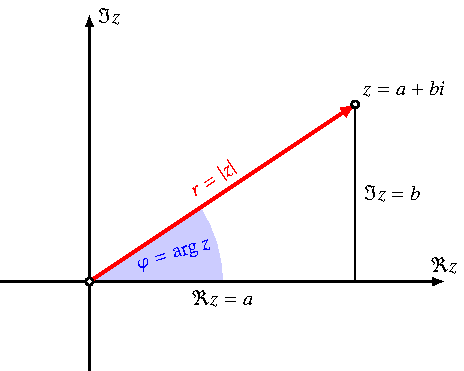
\includegraphics{chapters/05-zahlen/images/komplex.pdf}
\caption{Argument und Betrag einer komplexen Zahl $z=a+ib$ in der 
Gaussschen Zahlen\-ebene
\label{buch:zahlen:cfig}}
\end{figure}%

Die Zahlenebene führt auf eine weitere mögliche Parametrisierung einer
komplexen Zahl.
Ein Punkt $z$ der Ebene kann in Polarkoordinaten auch durch den {\em Betrag}
\index{Betrag}%
\index{Polarkoordinaten}%
und den Winkel zwischen der reellen Achse und dem Radiusvektor zum Punkt,
dem sogenannten {\em Argument},
charakterisiert werden.

\subsubsection{Komplexe Konjugation}
Der komplexen Zahl $u=a+bi$ ordnen wir die sogenannte
{\em komplex konjugierte} Zahl $\overline{z} = a-bi$ zu.
Mit Hilfe der komplexen Konjugation $z\mapsto\overline{z}$
kann man den Real- und Imaginärteil
\index{komplexe Konjugation}%
\index{Konjugation, komplexe}%
algebraisch ausdrücken:
\[
\Re z 
=
\frac{z+\overline{z}}2
=
\frac{a+bi+a-bi}{2}
=
\frac{2a}2
=a
\qquad\text{und}\qquad
\Im z
=
\frac{z-\overline{z}}{2i}
=
\frac{a+bi-a+bi}{2i}
=
\frac{2bi}{2i}
=
b.
\]
In der Gaussschen Zahlenebene ist die komplexe Konjugation eine
Spiegelung an der reellen Achse.

\subsubsection{Betrag}
In $\mathbb{R}$ kann man die Ordnungsrelation dazu verwenden zu entscheiden,
ob eine Zahl $0$ ist. 
Wenn $x\ge 0$ ist und $x\le 0$, dann ist $x=0$.
In $\mathbb{C}$ steht diese Ordnungsrelation nicht mehr zur Verfügung.
Eine komplexe Zahl ist von $0$ verschieden, wenn die Länge des Vektors in der
Zahlenebene verschieden von $0$ ist.
Wir definieren daher den {\em Betrag} einer komplexen Zahl $z=a+bi$ als
\index{Betrag}
\[
|z|^2
=
a^2 +b^2
=
(\Re z)^2 + (\Im z)^2
\qquad\Rightarrow\qquad
|z|
=
\sqrt{a^2+b^2}
=
\sqrt{(\Re z)^2 + (\Im z)^2}.
\]
Der Betrag lässt sich auch mit Hilfe der komplexen Konjugation ausdrücken,
es ist $z\overline{z} = (a+bi)(a-bi) = a^2+abi-abi+b^2 = |z|^2$.
Der Betrag ist immer eine reelle Zahl.

\subsubsection{Division}
Die Erweiterung zu den komplexen Zahlen muss auch die Division erhalten.
Dies ist durchaus nicht selbstverständlich.
Man kann zeigen, dass ein Produkt von Vektoren eines Vektorraums nur für
einige wenige, niedrige Dimensionen überhaupt möglich ist.
Für die Division sind die Einschränkungen noch gravierender, die einzigen
Dimensionen $>1$, in denen ein Produkt mit einer Division definiert werden
kann\footnote{Der Beweis dieser Aussage ist ziemlich schwierig und wurde
erst im 20.~Jahrhundert mit Hilfe der Methoden der algebraischen Topologie
erbracht. Eine Übersicht über den Beweis kann in Kapitel~10 von
\cite{buch:ebbinghaus} gefunden werden.}, sind $2$, $4$ und $8$.
Nur in Dimension $2$ ist ein kommutatives Produkt möglich, dies muss das
Produkt der komplexen Zahlen sein.

Wie berechnet man den Quotienten $\frac{z}{w}$ für zwei beliebige komplexe
Zahlen $z=a+bi$ und $w=c+di$ mit $w\ne 0$?
Dazu erweitert man den Bruch mit der komplex Konjugierten des Nenners:
\begin{align*}
\frac{z}{w}
&=
\frac{z\overline{w}}{w\overline{w}}
=
\frac{z\overline{w}}{|w|^2}
\end{align*}
Da der Nenner $|w|^2>0$ eine reelle Zahl ist, ist die Division einfach,
es ist die Multiplikation mit der reellen Zahl $1/|w|^2$.

Wir können den Quotienten auch durch Real- und Imaginärteil ausdrücken:
\begin{align*}
\frac{z}{w}
&=
\frac{a+bi}{c+di}
=
\frac{(a+bi)(c+di)}{(c+di)(c-di)}
=
\frac{ac-bd +(ad+bc)i}{c^2+d^2}.
\end{align*}


\subsubsection{Geometrische Interpretation der Rechenoperationen}
Die Addition komplexer Zahlen wurde bereits als Vektoraddition
in der Gausschen Zahlenebene interpretiert. 
Die Multiplikation ist etwas komplizierter, wir berechnen Betrag
und Argument von $zw$ separat.
Für den Betrag erhalten wir
\begin{align*}
|zw|^2
&=
zw\overline{(zw)}
=
zw\overline{z}\overline{w}
=
z\overline{z}w\overline{w}
=
|z|^2|w|^2
\end{align*}
Der Betrag des Produktes ist also das Produkt der Beträge.

Für das Argument verwenden wir, dass
\[
\tan\operatorname{arg}z
=
\frac{\Im z}{\Re z}
=
\frac{b}{a}
\qquad\Rightarrow\qquad
b=a\tan\operatorname{arg}z
\]
und analog für $w$.
Bei der Berechnung des Produktes behandeln wir nur den Fall $a\ne 0$ 
und $c\ne 0$, was uns ermöglicht, den Bruch durch $ac$ zu kürzen:
\begin{align*}
\tan\arg wz
&=
\frac{\Im wz}{\Re wz}
=
\frac{ad+bc}{ac-bd}
=
\frac{\frac{d}{c} + \frac{b}{a}}{1-\frac{b}{a}\frac{d}{c}}
=
\frac{
\tan\operatorname{arg}z+\tan\operatorname{arg}w
}{
1+
\tan\operatorname{arg}z\cdot\tan\operatorname{arg}w
}
=
\tan\bigl(
\operatorname{arg}z+\operatorname{arg}w
\bigr).
\end{align*}
Im letzten Schritt haben wir die Additionsformel für den Tangens verwendet.
\index{Additionstheorem für Tangens}%
Daraus liest man ab, dass das Argument eines Produkts die Summe der
Argumente ist.
Die Multiplikation mit einer festen komplexen Zahl führt also mit der ganzen
komplexen Ebene eine Drehstreckung durch.
Auf diese geometrische Beschreibung der Multiplikation werden wir zurückkommen,
wenn wir die komplexen Zahlen als Matrizen beschreiben wollen.

\subsubsection{Algebraische Vollständigkeit}
Die komplexen Zahlen $\mathbb{C}$ sind als Erweiterung von $\mathbb{R}$
so konstruiert worden, dass die Gleichung $x^2+1=0$ eine Lösung hat.
Etwas überraschend ist dagegen, dass in dieser Erweiterung jetzt jede
beliebige algebraische Gleichung lösbar geworden ist.
Dies ist der Inhalt des Fundamentalsatzes der Algebra.

\begin{satz}[Fundamentalsatz der Algebra]
\label{buch:zahlen:satz:fundamentalsatz}
\index{Fundamentalsatz der Algebra}%
Jede algebraische Gleichung der Form
\[
p(x)=x^n + a_{n-1}x^{n-1}+a_1x+a_0=0,\qquad a_k\in\mathbb{C}
\]
mit komplexen Koeffizienten hat $n$ möglicherweise mit Vielfachheit
gezählte Nullstellen $\alpha_1,\dots,\alpha_m$, d.~h.~das Polynom $p(x)$
lässt sich in Linearfaktoren
\[
p(x)
=
(x-\alpha_1)^{k_1}(x-\alpha_2)^{k_2}\cdot\ldots\cdot(x-\alpha_m)^{k_m}
\]
zerlegen, wobei $k_1+k_2+\dots+k_m=n$.
Die Zahl $k_j$ heisst die {\em Vielfachheit} der Nullstelle $\alpha_j$.
\end{satz}

Der Fundamentalsatz der Algebra wurde erstmals von Carl Friedrich Gauss
\index{Gauss, Carl Friedrich}%
vollständig bewiesen.
Seither sind viele alternative Beweise mit Methoden aus den verschiedensten
Gebieten der Mathematik gegeben worden.
Etwas salopp könnten man sagen, dass der Fundamentalsatz ausdrückt, dass
die Konstruktion der Zahlensysteme mit $\mathbb{C}$ abgeschlossen ist,
soweit damit die Lösbarkeit beliebiger Gleichungen angestrebt ist.

\subsubsection{Quaternionen und Octonionen}
Die komplexen Zahlen ermöglichen eine sehr effiziente Beschreibung 
geometrischer Abbildungen wie Translationen, Spiegelungen und 
Drehstreckungen in der Ebene.
Es drängt sich damit die Frage auf, ob sich $\mathbb{C}$ so erweitern
lässt, dass man damit auch Drehungen im dreidimensionalen Raum
beschreiben könnte.
Da Drehungen um verschiedene Achsen nicht vertauschen, kann eine solche
Erweiterung nicht mehr kommutativ sein.

William Rowan Hamilton propagierte ab 1843 eine Erweiterung von $\mathbb{C}$
\index{Hamilton, William Rowan}%
mit zwei zusätzlichen Einheiten $j$ und $k$ mit den nichtkommutativen
Relationen
\begin{equation}
i^2 = j^2 = k^2 = i\!jk = -1.
\label{buch:zahlen:eqn:quaternionenregeln}
\end{equation}
Er nannte die Menge aller Linearkombinationen 
\[
\mathbb{H} = \{ a_0+a_1i+a_2j+a_3k\;|\; a_l\in \mathbb{R}\}
\]
die {\em Quaternionen}, die Einheiten $i$, $j$ und $k$ heissen auch
\index{Quaternionen}%
Einheitsquaternionen.
\index{Einheitsquaternionen}%
Konjugation, Betrag und Division können ganz ähnlich wie bei den
\index{Konjugation von Quaternionen}%
\index{Betrag einer Quaternion}%
\index{Division durch eine Quaternion}%
komplexen Zahlen definiert werden und machen $\mathbb{H}$ zu einer
sogenannten {\em Divisionsalgebra}.
\index{Divisionsalgebra}%
Alle Rechenregeln mit Ausnahme der Kommutativität der Multiplikation
sind weiterhin gültig und durch jede von $0$ verschiedene Quaternion
kann auch dividiert werden.

Aus den Regeln für die Quadrate der Einheiten in
\eqref{buch:zahlen:eqn:quaternionenregeln} folgt zum Beispiel
$i^{-1}=-i$, $j^{-1}=-j$ und $k^{-1}=-k$.
Die letzte Bedingung liefert daraus
\[
i\!jk=-1
\qquad\Rightarrow\qquad
\left\{
\quad
\begin{aligned}
i\!j
&=
i\!jkk^{-1}=-1k^{-1}=k
\\
i^2\!jk&=-i=-jk
\\
-j^2k&=-ji=k
\end{aligned}
\right.
\]
Aus den Relationen~\eqref{buch:zahlen:eqn:quaternionenregeln}
folgt also insbesondere auch, dass $i\!j=-ji$.
Ebenso kann abgeleitet werden, dass $jk=-k\!j$ und $ik=-ki$.
Man sagt, die Einheiten sind {\em antikommutativ}.
\index{antikommutativ}%

Die Beschreibung von Drehungen mit Quaternionen ist in der
Computergraphik sehr beliebt, weil eine Quaternion mit nur vier
Komponenten $a_0,\dots,a_3$ vollständig beschrieben ist.
Eine Transformationsmatrix des dreidimensionalen Raumes enthält
dagegen neun Koeffizienten, die vergleichsweise komplizierte 
Abhängigkeiten erfüllen müssen.
Kapitel~\ref{chapter:clifford} behandelt nicht nur die Beschreibung
von Drehungen des dreidimensionalen Raumes sondern eine weitreichende
Verallgemeinerung dieser Idee, die sogenannte {\em geometrische Algebra}.
\index{geometrische Algebra}%
Quaternionen haben auch in weiteren Gebieten interessante Anwendungen,
zum Beispiel in der Quantenmechanik, wo antikommutierende Operatoren
\index{Quantenmechanik}%
bei der Beschreibung von Fermionen eine zentrale Rolle spielen.
\index{Fermion}%

Aus rein algebraischer Sicht kann man die Frage stellen, ob es eventuell
auch noch grössere Divisionsalgebren gibt, die $\mathbb{H}$ erweitern.
Tatsächlich hat Arthur Cayley 1845 eine achtdimensionale Algebra,
die Oktonionen $\mathbb{O}$, mit vier weiteren Einheiten beschrieben.
\index{Cayley, Arthur}%
Allerdings sind die Oktonionen nur beschränkt praktisch anwendbar.
Grund dafür ist die Tatsache, dass die Multiplikation in $\mathbb{O}$
nicht mehr assoziativ ist.
Das Produkt von mehr als zwei Faktoren aus $\mathbb{O}$ ist von der
Reihenfolge der Ausführung der Multiplikationen abhängig.








%\section*{Übungsaufgaben}
%\aufgabetoplevel{chapters/05-zahlen/uebungsaufgaben}
%\begin{uebungsaufgaben}
%\end{uebungsaufgaben}

